\section{Tuning non-linear filters}

For this part, mainly use the code from question 2 a and b. 

Firstly, Draw the figure containing the true positions, filtered positions, sensor positions, the measurements, $ 5 \sigma $ curves,  and the true position sequence. This figure can very graphically tell us the tracking effect of the filter and the general covariance.

Secondly, draw the histogram of the error. This can help us evaluate the quality of the filter.

\subsection{a}
\subsubsection{Tuning big}

$\sigma_v$=1 $\sigma_w$=pi/180

\begin{figure}[H]
 \centering
 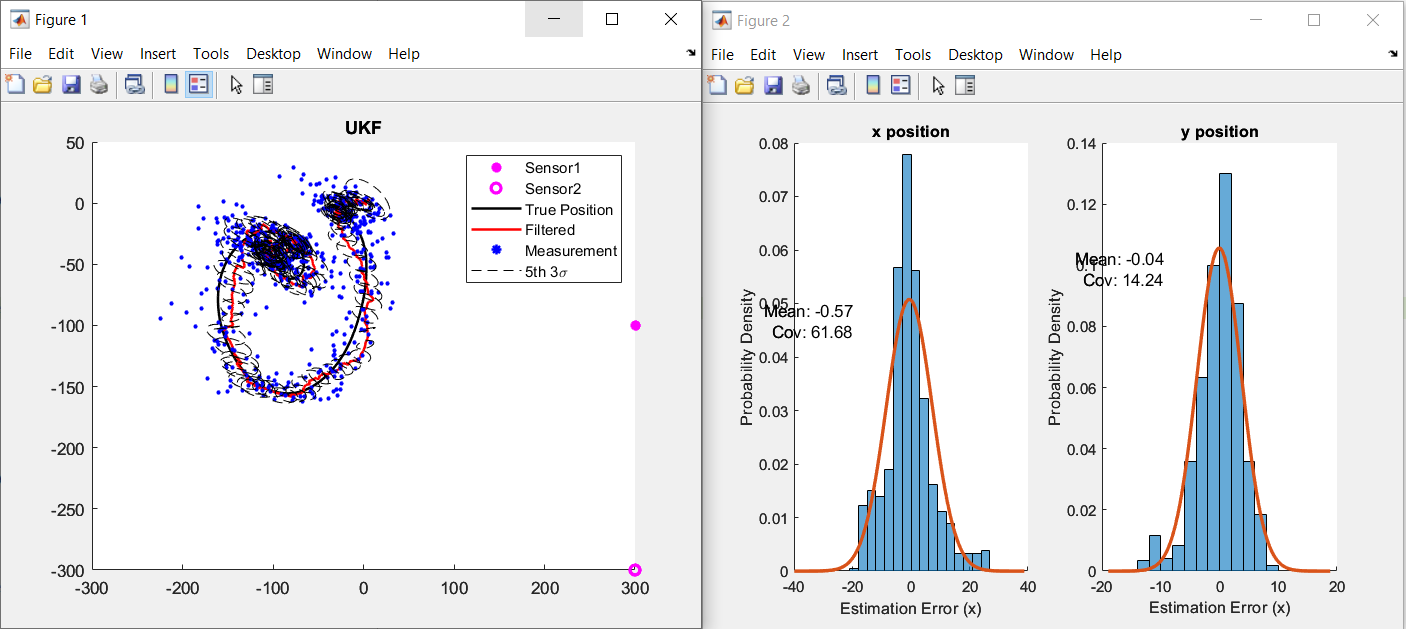
\includegraphics[width=0.7\textwidth]{images/begin.png}
 \caption{Begin Value}
 \label{31}
\end{figure}

\begin{figure}[H]
 \centering
 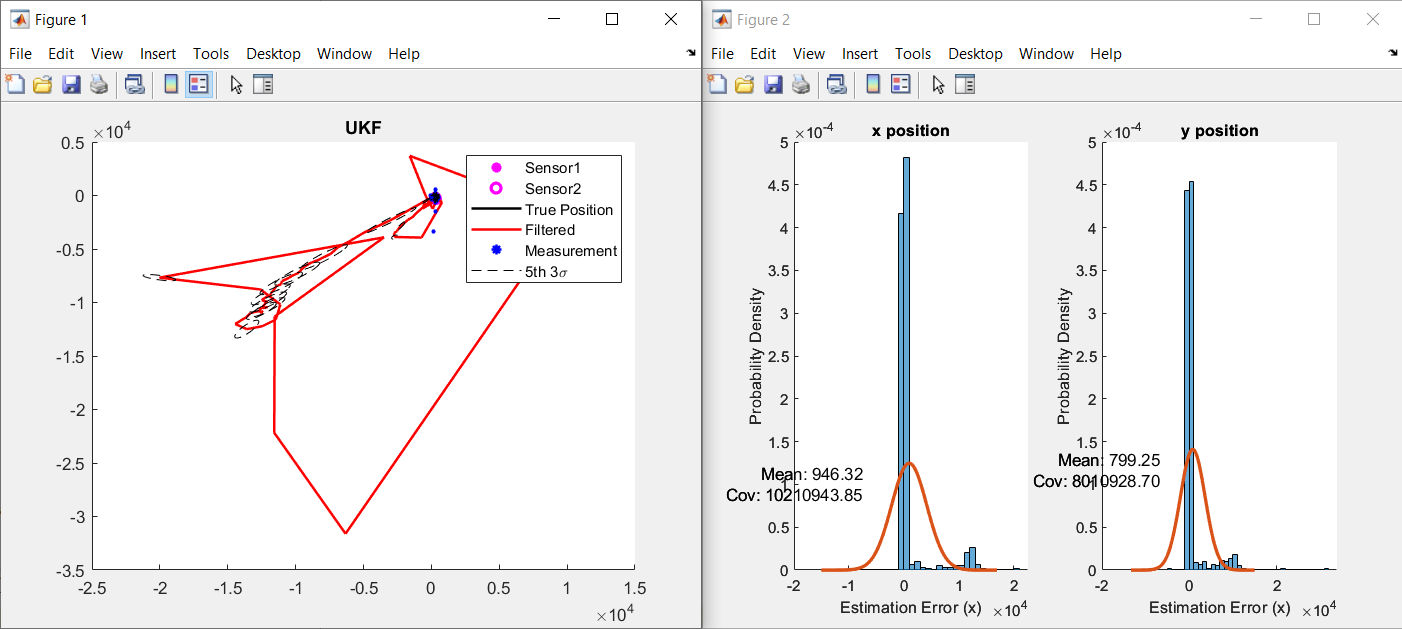
\includegraphics[width=0.7\textwidth]{images/sigmav1000.png}
 \caption{$\sigma_v$ times 1000, $\sigma_w$ keeps 1}
 \label{v1000}
\end{figure}

Firstly use large process noise, which means the filter now do not believe the state velocity from motion model, and it can now track the true state.

\begin{figure}[H]
 \centering
 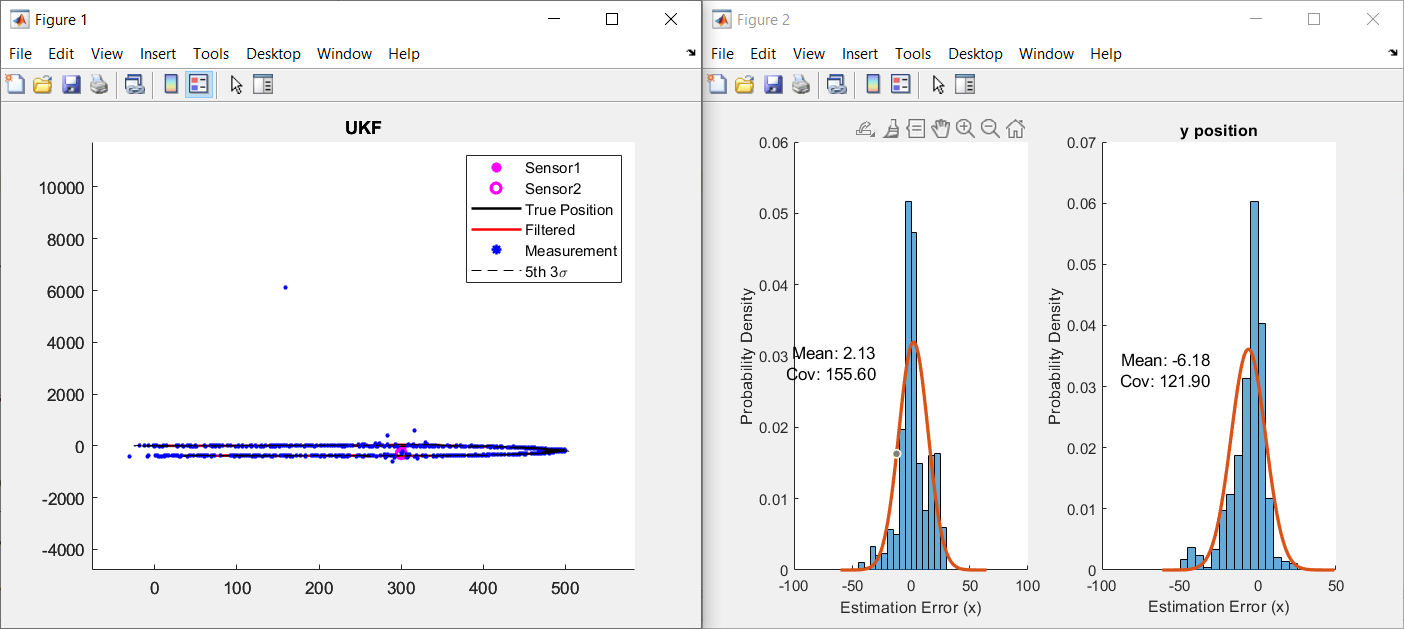
\includegraphics[width=0.7\textwidth]{images/sigmaw1000.png}
 \caption{$\sigma_w$ times 1000}
 \label{w1000}
\end{figure}

Then use large $\sigma_w$, which means the filter now do not believe the rotation speed of the motion model, it can still track the true state, since the tracking states are positions not the gesture. But it still make the filter quality worser.

Then increase both, we should see the seem result with only increase $\sigma_v$

\begin{figure}[H]
 \centering
 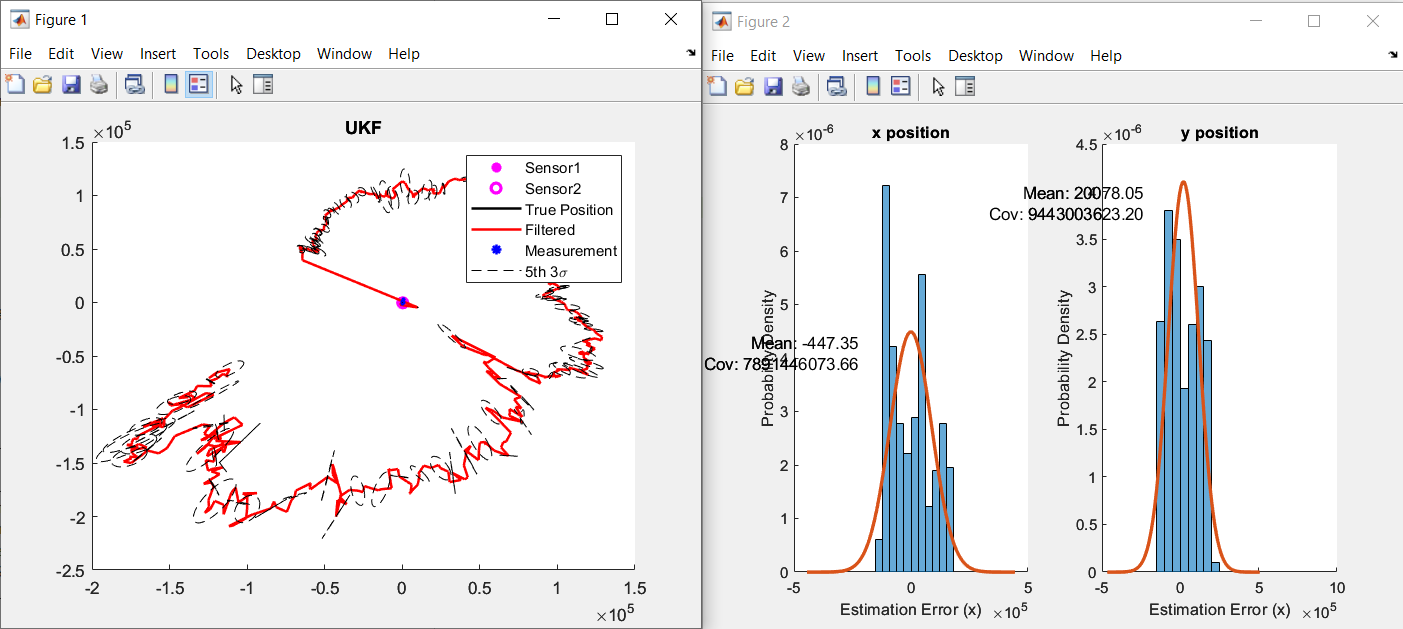
\includegraphics[width=0.7\textwidth]{images/both.png}
 \caption{Both times 1000}
 \label{both1000}
\end{figure}

And it fits my guess.

\subsection{Tuning down}

From tuning big part, I guess turn the $\sigma_v$ down enhance the quality, while $ \sigma_w $  only matter a little.

\begin{figure}[H]
 \centering
 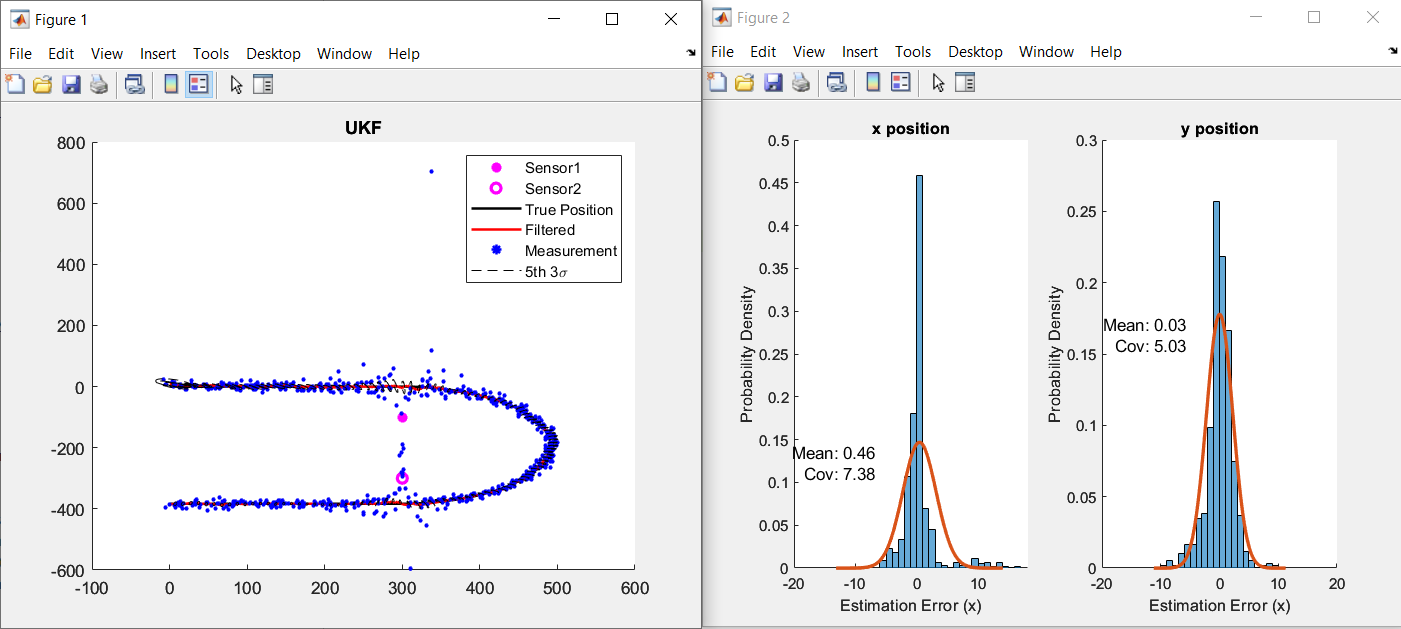
\includegraphics[width=0.7\textwidth]{images/1e3sigmav.png}
 \caption{$\sigma_v/1000$}
 \label{1e-3sigmav}
\end{figure}

\begin{figure}[H]
 \centering
 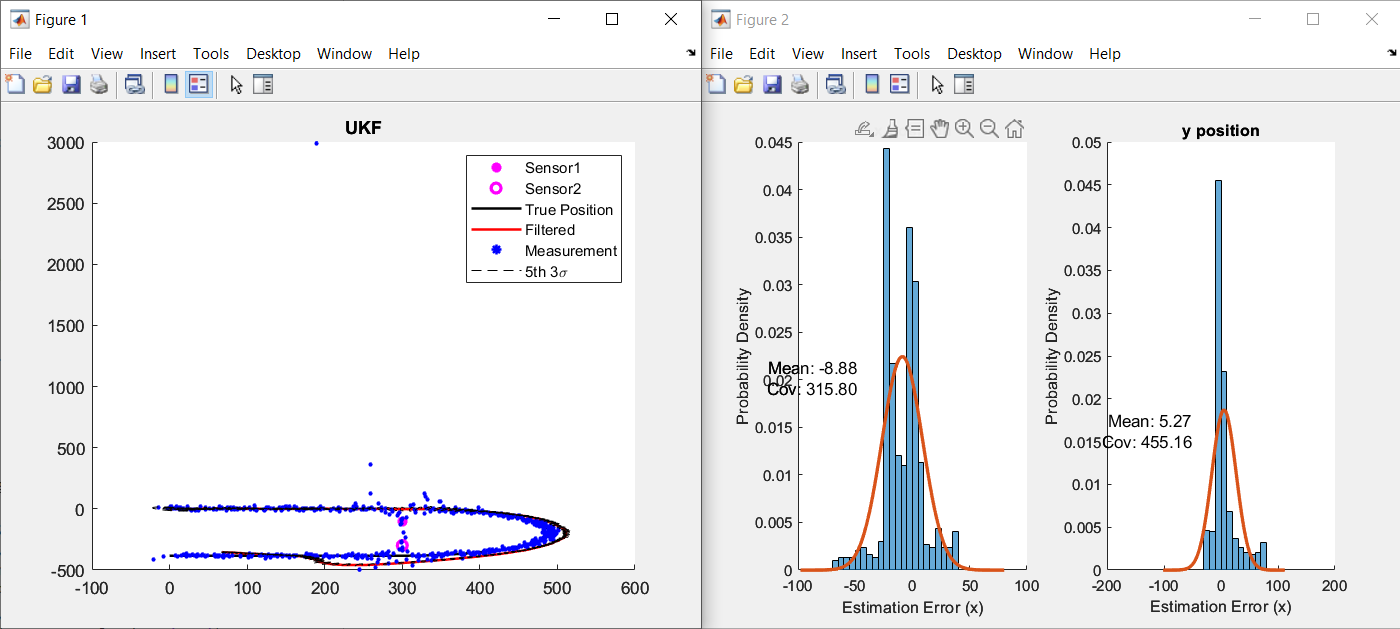
\includegraphics[width=0.7\textwidth]{images/1e-3sigamw.png}
 \caption{$\sigma_w/1000$}
 \label{1e-3sigamw}
\end{figure}

\begin{figure}[H]
 \centering
 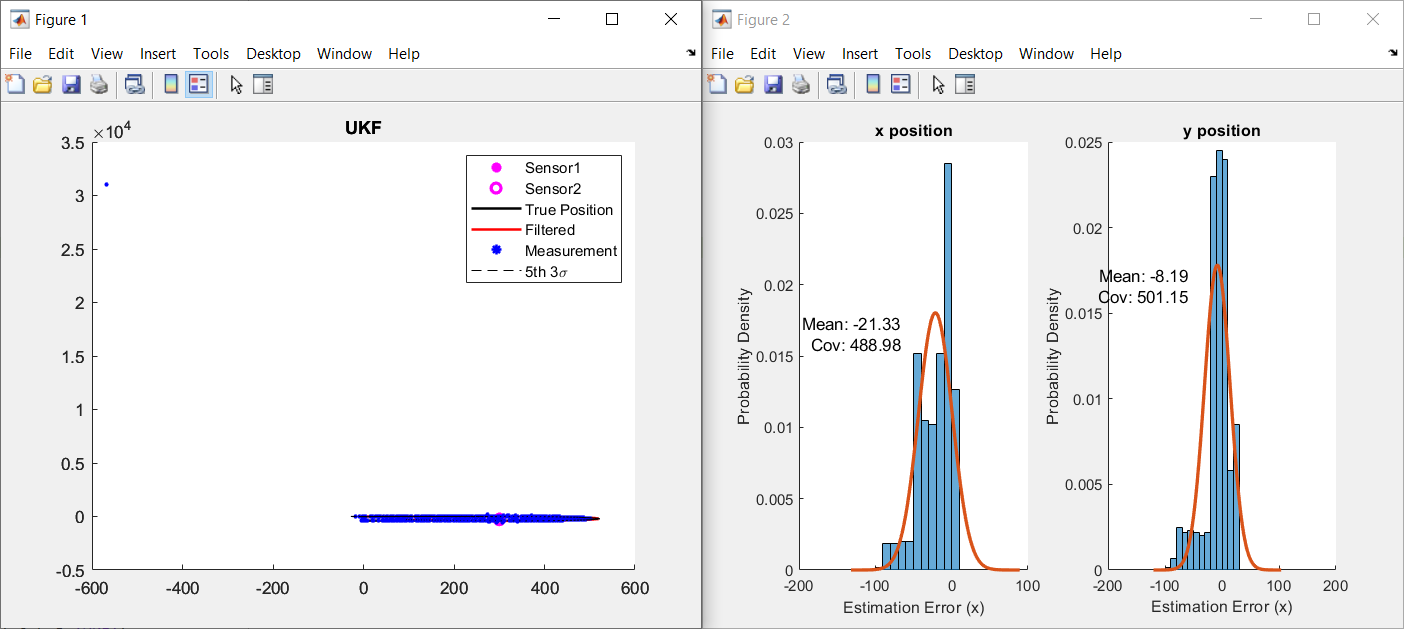
\includegraphics[width=0.7\textwidth]{images/both1e-3.png}
 \caption{Both / 1000}
 \label{both1e-3}
\end{figure}

But my guess is not fully correct. Now the motion covariances are two small that we only believe the motion model, which make the system lag behind the change.

When both parameters are really small, the filter quality drops.

\subsection{b}
I tuned $\sigma_v$ as $50$ and $\sigma_w$ as $pi/180*60$. Under these parameters the filer can always track the true state and the mean and covariance of the state x is better then the beginning value.
\begin{figure}[H]
 \centering
 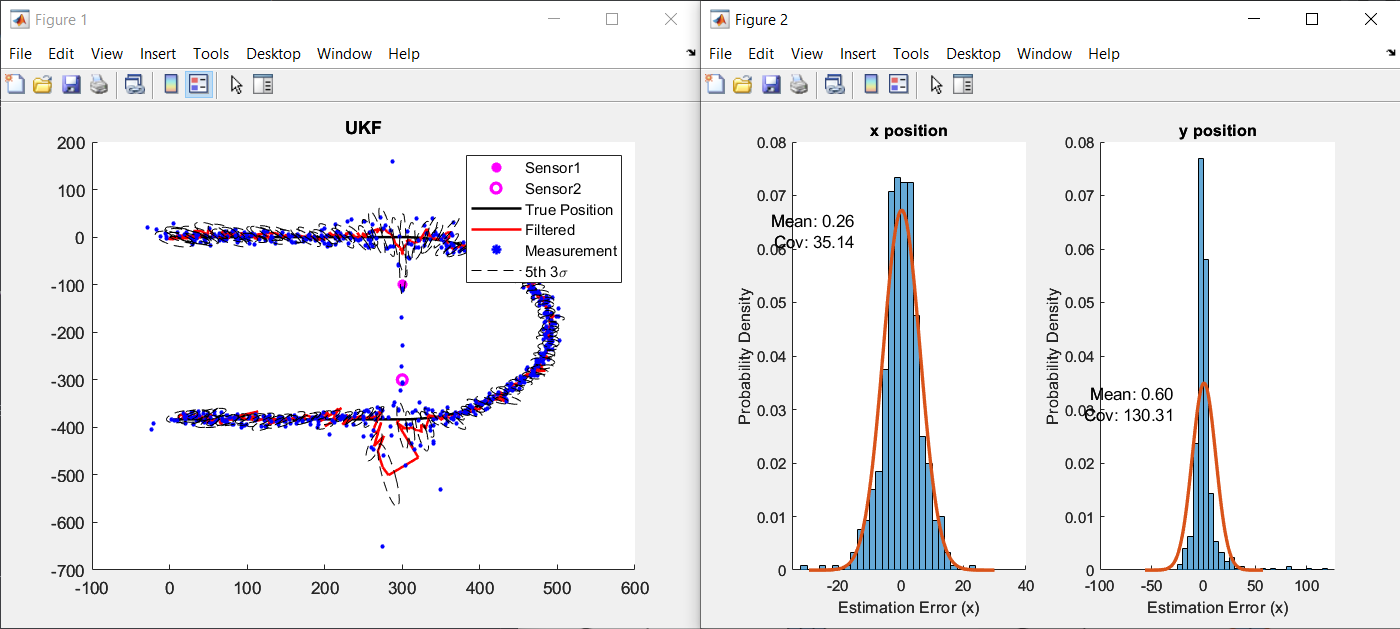
\includegraphics[width=0.7\textwidth]{images/mytune.png}
 \caption{Mytune}
 \label{mytune}
\end{figure}

\subsection{c}

\begin{figure}[H]
 \centering
 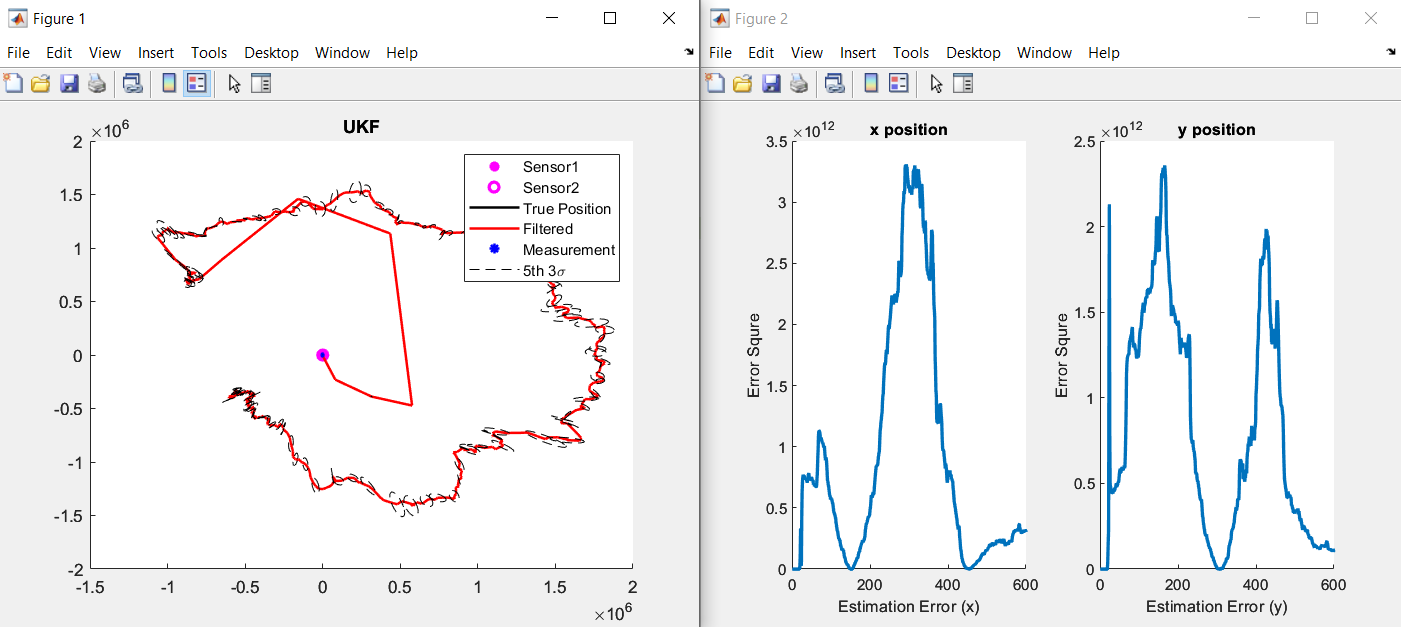
\includegraphics[width=0.7\textwidth]{images/toobig.png}
 \caption{Toobig: Both times 1000 1000}
 \label{toobig}
\end{figure}

\begin{figure}[H]
 \centering
 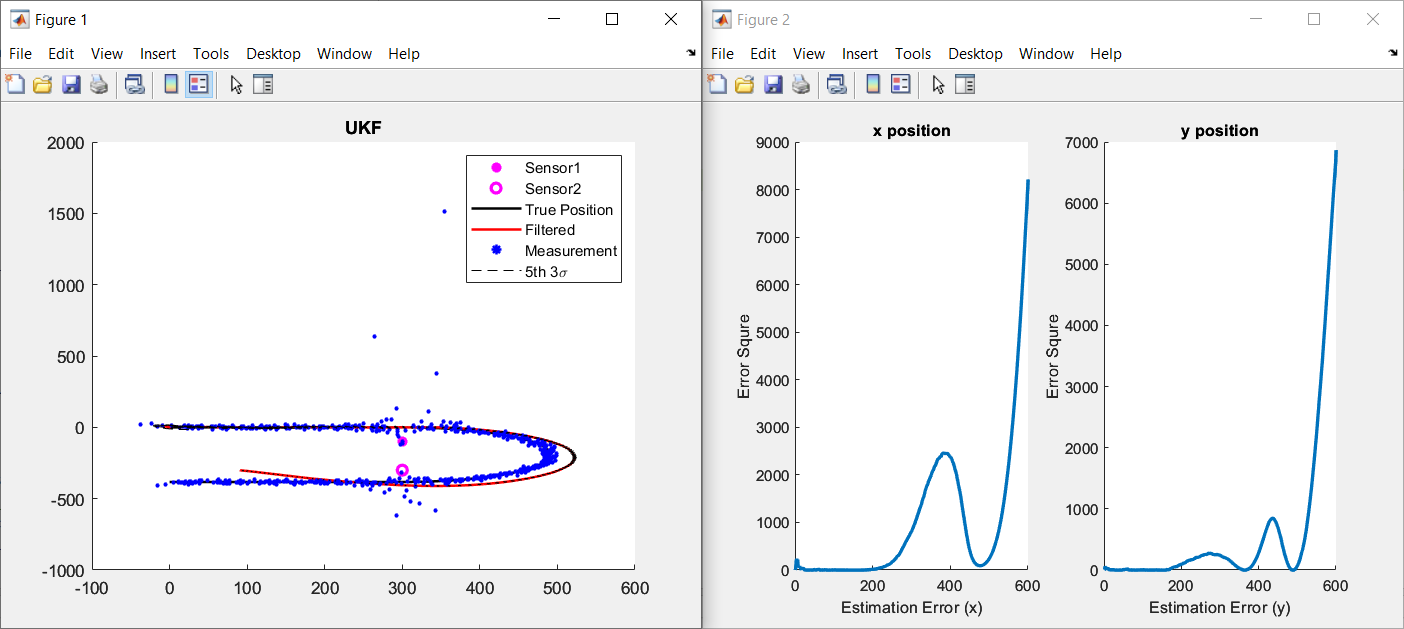
\includegraphics[width=0.7\textwidth]{images/toosmall.png}
 \caption{Too small: Both are divided by 1000}
 \label{toosmall}
\end{figure}

\begin{figure}[H]
 \centering
 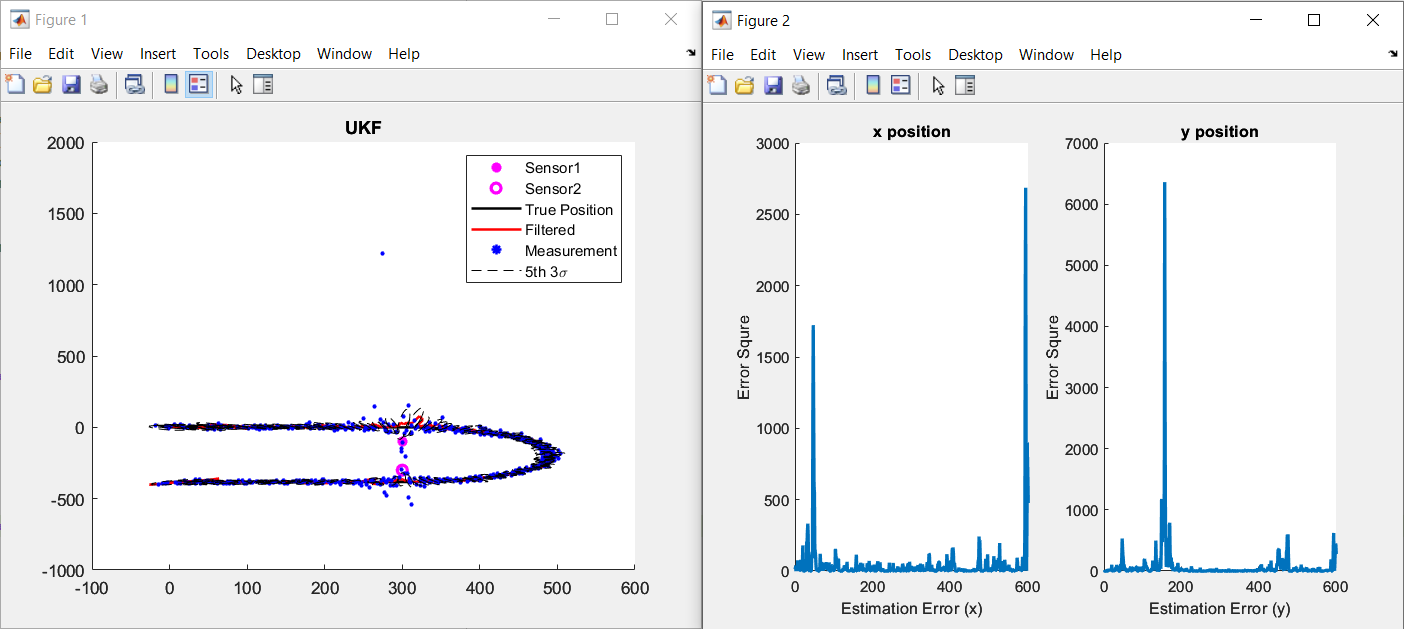
\includegraphics[width=0.7\textwidth]{images/welltuned.png}
 \caption{Welltuned}
 \label{welltune}
\end{figure}

From figures above, it is obvious that the well tuned one has the minimum average position errors, which means it perform the best, and matches the left side state curve.

\subsection{d}

It is not possible to have accurate estimates over the whole sequence. Since we have turn in the true state, we need flexibility to follow this trun, or we will loose the track of the true state.


There is a conflict when tuning for different parts of the true trajectory, for in some parts the system do not change its state that the parameters can set very small while in some parts the car may turn direction, need bigger parameters.


We would set a much smaller parameter for a completely straight line, and a much larger parameter for a purely turning session.

For changing from straight to turn, since it generally picks up more changes after this operation, I think its parameter should be larger to get more flexibility than changing from turn to straight, which may keep driving in a straight line.

To conclusion, the purpose of introducing motioin covariance into the motion model is to increase the flexibility of the system and to make it robust enough to cope with changes such as sudden acceleration and steering of the vehicle.

It is true that we can get very small error for a given case, but this is not migratory at all and is a meaningless behavior.